\section{The \lang language}

\lang is a minimal ML-like language with
let-polymorphism, abstract types, and pairs. Its type system manages
linearity and borrows using kinds and (kind-) constrained types.
For ease of presentation, we keep the language as simple as possible.
\begin{itemize}
\item We showcase pattern matching on pairs rather than algebraic
  datatypes.
\item We have separate operators for borrowing and reborrowing (taking
  the borrow of a borrow).
\item We assume that regions are explicit in the code. (But we present
  an algorithm to infer them in \cref{regionannot}.)
\item We use de Bruijn-indexing to identify regions instead of region
  variables. 
\end{itemize}

The rest of this section formalizes  \lang: the syntax (\cref{syntax}),
the statics in terms of syntax directed typing (\cref{sdtyping}),
and a dynamics that is linearity-aware (\cref{sem}).

\subsection{Syntax}
\label{syntax}


\Cref{grammar} defines the syntax of \lang. Expressions are as usual
in an ML-like language.  The novel aspects are match
specifications, regions, and borrows.

We start from the bottom.
A borrow $\borrow{x}$ is always taken from a variable $x$. The
\emph{borrow annotation} $\BORROW$ indicates whether the borrow is mutable
($\MBORROW$) or immutable ($\IBORROW$). If $x$ is already borrowed,
then we need to use the reborrow expression $\reborrow{x}$.

A region $\region{\Sone x\BORROW}{e}$ is annotated with its nesting $n$, the variable $x$ that may be borrowed in $e$, and the kind of borrow $\BORROW$.

A match is indexed with a \emph{match specification} $\etransfm$ that indicates
whether the match should work on borrows ($\etransfm=\&^b$) or not ($\etransfm=id$).

Many types are indexed with kinds, ranged over by $k$.
A kind is either a kind variable $\kvar$ or a constant
(linear $\klin$, affine $\kaff$, or unrestricted $\kun$) indexed
by a nesting level $n \in \Nat \cup \{\infty\}$.

A type $\tau$ is either a type variable, a function type indexed by a
kind, 
a type application $\tapp{t}{\Multi{\tau}}$ of an abstract type constructor
$\T t$, or a borrowed type  $\borrowty{k}{\tau}$.

Type schemes $\schm$ add quantification over kind
variables $\kappa$, kinded type variables $\alpha:k$, and constraints
$C$ to a type, where a constraint is a list of inequalities over
kinds.

Abstract type constructors possess kind schemes $\kschm$ which relate
the kinds of the type constructors arguments to the kind of the
constructed type.

Generally, we write lists with an overbar and (sometimes) an index as
in $\Multi[i]\tau$.

% \paragraph{Previously}


% Let us first define our conventions and meta-syntactic variables.
% Expressions, types and kinds are noted respectively $e$, $\tau$, and $k$.
% Variables, type variables and kind variables are noted
% respectively $x$, $\tvar$ and $\kvar$. Types and kind schemes
% are noted $\schm$ and $\kschm$.
% In the rest of the text, we will write lists with a bar and an index, for
% instance $\Multi[i]{\tau}$.
% Kind constants are noted in bold capital letters, such as $\kaff$ for affine.

% The syntax of \lang is presented in \cref{grammar} and follows
% traditional ML languages with let bindings.
% Borrows, noted $\borrow{e}$, are annotated with a specification indicating
% if a borrow is immutable ($\IBORROW$) or mutable ($\MBORROW$).
% We also distinguish reborrows, which are noted $\reborrow{e}$.
% Match are indexed with a specification which can be either $\&^b$
% (which $b$ a borrow specification) or $id$, indicating if the match
% should operate on borrows or not.
% Regions, noted $\region{\Sone x\BORROW}{e}$ are annotated with their nesting ($n$)
% and the variable whose borrow they enclose ($x$).
% %
% $\tapp{t}{\Multi{\tau}}$ denotes a type application where
% $\T t$ is an abstract type constructor.
% Arrow and borrow types are annotated with a kind, noted $\tau \tarr{k} \tau$
% and $\borrowty{k}{\tau}$ respectively.
% %
% Kinds can be either a kind variable $\kvar$, or constants
% (linear $\klin$, affine $\kaff$ or unrestricted $\kun$) indexed
% by a nesting level represented by a member of $N \cup \{\infty\}$.
% Type schemes and kind schemes are guarded by a set of constraints.
% %
% Finally, constraints are composed of a list of kind inequalities.

% Environments are composed of value and type bindings, along with type
% declarations. Type declarations, of the form
% $\tydecl{t}{\kschm}{K}{\tau}$, introduce both a new type constructor $\T{t}$ and
% a data constructor $K$.

\begin{figure*}[t]
  \centering
  \begin{subfigure}[t]{0.45\linewidth}
\begin{align*}
  \htag{Expressions}
  e ::=&\ c \mid x \mid \app{e}{e'} \mid \lam{x}{e} \mid \letin{x}{e}{e'}\\
  % |&\ \fix{e}\tag{Fixpoint}\\
  |&\ \introPair{e}{e'} \mid \matchin{x,y}{e}{e'}\tag{Pairs}\\
  |&\ \region{x}{e}\tag{Region}\\
  |&\ \borrow{x}\tag{Borrows}\\
  % |&\ \introK{K}{e}\tag{Data Constructor introduction}\\
  % |&\ \elimK{K}{e}\tag{Data Constructor elimination}\\
  \htag{Environments}
  \E ::=&\ b^*\\
  b ::=&\ \bvar{x}{\schm}\tag{Variable bindings}\\
  |&\ \bvar{\tvar}{\kschm}\tag{Type bindings}\\
  % |&\ \tydecl{t}{\kschm}{K}{\tau}\tag{Type Declaration}\\
  \htag{Type and kind Schemes}
  \schm ::=&\ \forall\kvar^*\forall\bvar{\alpha}{k}^*.(\qual{C}{\tau})\\
  \kschm ::=&\ \forall\kvar^*.(\qual{C}{k_i^* \karr k})\\
\end{align*}
\end{subfigure}\hfill
\begin{subfigure}[t]{0.5\linewidth}
\begin{align*}
  \htag{Type Expressions}
  \tau ::=&\ \tvar\tag{Type variables}\\
  |&\ \tau\tarr{k}\tau\tag{Function types}\\
  |&\ \tapp{t}{\tau^*}\tag{Type constructors}\\
  |&\ \borrow{\tau}\tag{Borrowed Type}\\
  \htag{Kinds}
  k ::=&\ \kvar\tag{Kind variables}\\
  |&\ \klin_n\tag{Linear kind}\\
  |&\ \kaff_n\tag{Affine kind}\\
  |&\ \kun_n\tag{Unrestricted kind}\\
  n \in&\ \mathbb N \cup \{\infty\}\\
  \htag{Constraints}
  C ::= (\Cleq{k}{k'})^*
\end{align*}
\end{subfigure}

%%% Local Variables:
%%% mode: latex
%%% TeX-master: "main"
%%% End:

  \caption{Syntax}
  \label{grammar}
\end{figure*}

\subsection{Typing}
\label{sdtyping}

We now present the essential parts of our \lang's type system. A complete
description of the system is available in \cref{appendix:sdtyping}.
In this section, we focus on chosen parts of our system
through a set of selected rules.
%
We introduce the following typing, kinding and constraint judgements:
\begin{description}
\item[$\inferS{C}{\E}{e}{\tau}$ --]
  Expression $e$ has type $\tau$ in environment $\E$ under constraints $C$.
\item[$\inferSK{C}{\E}{\tau}{k}$ --]
  Type $\tau$ has kind $k$ in environment $\E$ under constraints $C$.
\item[$\entail{D}{C}$ --] Constraint $D$ implies constraint $C$.
\end{description}

\subsubsection{Kinds and constraints}

One novel feature or \affe is the use of kinds and qualified types to encode
linear and affine types. Before explaining the details of our type system, we
give a quick presentation of the kinds and constraints.
A kind $k$ can be either a kind variable, $\kvar$, or a constant.
Each constant is composed of a ``quality'' and a ``level''.
The quality describes the use pattern of the type and can be
either unrestricted $\kun$, affine $\kaff$ or linear $\klin$. The level
describes the nested regions in which it can be used. Levels are represented
by a natural number of $\infty$.
$0$ represents the normal scope outside of any region and is often omitted
(for instance $\kaff_0$ is simply noted $\kaff$).
$\infty$ is the empty region that is infinitely nested and is mostly used
as an upper bound.
For instance, the constraint $\Cleq{\kvar}{\kun_\infty}$ indicates that
$\kvar$ must be unrestricted, but can be local to a region.
%
Just as presented before, constraints present in schemes and type signatures
are simply a list of atomic constraints, which are composed
of kind inequalities.
%
Our inequality constraints are based on an inequality relation on
kind constants noted $\lk_\Lat$. This relation forms a lattice
and  is summarized in
\cref{sdtyp:lattice}. We have the basic inequalities on qualities:
$\kun_n \lk_\Lat \kaff_n \lk_\Lat \klin_n$ for arbitrary regions $n$.
Additionally, the inequality follows the region nesting, for
instance $\kaff_n \lk_\Lat \kaff_{n+1}$.

\begin{figure*}[!h]
  \begin{minipage}{0.65\linewidth}
  \begin{mathpar}
    \inferrule[Lat-UAL]{}{\kun \lk \kaff \lk \klin}
    \and
    \inferrule[Lat-Level]{\mul \lk \mul' \and n \lk n'}{\mul_n \lk_\Lat \mul'_{n'}}
  \end{mathpar}
\end{minipage}~
\begin{minipage}{0.2\linewidth}
  \centering
  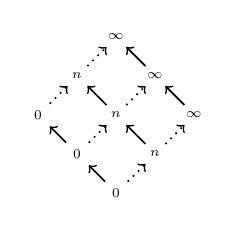
\begin{tikzpicture}
    [->,auto,semithick, every node/.style={scale=0.7}]
    \node(U) {$\kun_0$} ;
    \node(A) [above left of=U] {$\kaff_0$} ;
    \node(L) [above left of=A] {$\klin_0$} ;
    \node(Un) [above right of=U] {$\kun_n$} ;
    \node(An) [above left of=Un] {$\kaff_n$} ;
    \node(Ln) [above left of=An] {$\klin_n$} ;
    \node(Uinf) [above right of=Un] {$\kun_\infty$} ;
    \node(Ainf) [above left of=Uinf] {$\kaff_\infty$} ;
    \node(Linf) [above left of=Ainf] {$\klin_\infty$} ;
    \path
    (U) edge (A)
    (A) edge (L)
    (Un) edge (An)
    (An) edge (Ln)
    (Uinf) edge (Ainf)
    (Ainf) edge (Linf)
    ;
    \path[dotted]
    (U) edge (Un)
    (A) edge (An)
    (L) edge (Ln)
    (Un) edge (Uinf)
    (An) edge (Ainf)
    (Ln) edge (Linf)
    ;
  \end{tikzpicture}
\end{minipage}

%%% Local Variables:
%%% mode: latex
%%% TeX-master: "../main"
%%% End:

  \caption{Lattice inequalities -- $k \lk_\Lat k'$}
  \label{sdtyp:lattice}
\end{figure*}


\subsubsection{Environments and bindings}
\label{sdtyping:envs}

\lang aims to control the usage of variables, either
through
linearity and affinity which restrict how variables are shared and ignored,
or through borrows which allow to circumvent the linearity rules
in a controlled way.
In order to check these properties, we introduce several new bindings
in our typing environments.
The grammar of type environment (noted $\E$) is shown in \cref{grammar:env}.
On top of the traditional type and value bindings, noted respectively
$\bvar{\tvar}{\kschm}$ and $\bvar{x}{\schm}$, we also consider two new
bindings.
Borrow bindings $\bvar{\borrow{x}}{\borrowty{k}{\tau}}$ indicates
that the borrow $\borrow{x}$ can be used directly, as implemented
by the rule {\sc Borrow} in \cref{selectrules:borrow}.
Suspended bindings, noted $\svar{x}{\schm}^n$, indicates that $x$
cannot be used immediately, but will be usable in a region
marked with $x$, which we detail in \cref{sdtyping:regions}.

Environments are also used to encode several linearity-related properties
through \emph{environment-wide constraints}.
Here we present how to control both unused variables and
closure captures through such environment constraints, noted $\Cleq{\E}{k}$.
The intuitive meaning of $\Cleq{\E}{k}$ is that for all bindings
$\bvar{x}{\tau}$ in $\E$,
if type $\tau$ has kind $k'$ (noted $\inferSK{C}{\E}{\tau}{k'}$)
then the following constraints should hold: $\Cleq{k'}{k}$.
While this definition is incomplete, it is sufficient to understand
its use in the {\sc Abs} and {\sc Var} rules shown in \cref{selectrules:binders}.
%
The {\sc Var} rule looks up the type scheme of the variable $x$ in
the environment $\E$
and instantiate a concrete type through the substitution $\unif$. It then
checks that the other bindings in $\E$ can safely be discarded by
ensuring they are not linear. This is achieved through the constraint
$\Cleq{\E\Sdel{x}}{\kaff_\infty}$ which replaces the traditional
``weakening'' rule found in many type systems.

The {\sc Abs} rule must ensures that if the body of the lambda captures
linear or affine variables, the content will be reflected in the kind
annotated on the arrow, such as $\tau_2 \tarr{k} \tau_1$.
In order to do so, we constraint all the bindings of $\E$ to be less than $k$.
If one of the binding of $\E$ contains a type whose kind is affine,
we will derive the constraints $\Cleq{\kaff}{k}$, which ensures that
the kind on the arrow is at least affine.
Note that $x$ is \emph{not} included in $\E$: since it's the argument of the
closure, its use should not induce a capture.

\begin{figure}[!h]
  \begin{minipage}{0.33\linewidth}
    \begin{align*}
      \E &::=\ \Eempty \mid \E;B\tag{Environments}\\
      B &::=\ \bnone \tag{Empty} \\
         &\mid \bvar{x}{\schm}\tag{Variables}\\
         &\mid \bvar{\borrow{x}}{\borrowty{k}{\tau}}\tag{Borrows}\\
         &\mid \svar{x}{\schm}^n \tag{Suspended}\\
         &\mid \bvar{\tvar}{\kschm}\tag{Types}
         % |&\ \tydecl{t}{\kschm}{K}{\tau}\tag{Type Declaration}\\
    \end{align*}
    \caption{Type environments}
    \label{grammar:env}
  \end{minipage}\hfill
  \begin{minipage}{0.65\linewidth}
    \begin{mathpar}
      \ruleSDBorrow
      \and
      \ruleSDLam
      \and
      \ruleSDVar
    \end{mathpar}
    \caption{The {\sc Borrow}, {\sc Abs} and {\sc Var} rules}
    \label{selectrules:borrow}
    \label{selectrules:binders}
  \end{minipage}
\end{figure}



\subsubsection{Copying and Splitting}
\label{sdtyping:split}

Linear and affine types also control the copy of variables.
To demonstrate how this is achieve in \lang, we show the
{\sc Pair} typing rule in \cref{sdtyp:pair}.
In the {\sc Pair} rule, we split the type environment $\E$ in two parts,
$\E_1$ and $\E_2$, which are used to typecheck the components of the pair.
We note the splitting $\lsplit{C}{\E}{\E_1}{\E_2}$ where $C$ is a constraint
that must be respected for the split to be valid.
The main splitting rules are shown in \cref{sdtyp:split}. Each
rule applies to a binding for a given variable. For instance, the
{\sc Both} rule indicates that if we can prove that $x$ is unrestricted, we
can duplicate it in both environments.
Similarly, since immutable borrows are always unrestricted, the
{\sc Borrow} rule allows to duplicate them arbitrarily.
The {\sc Left} and {\sc Right} rule allow to move a binding
to the left or right environment.
The {\sc Susp} and {\sc SuspB} allow to split off suspended bindings to
the left environment while conserving access to the binding on the right.
Such suspended binding can later be turned
into a borrow inside a region. The asymmetry here must always follow
the order of execution of the language: in \affe, execution is from left to
right, which means that a resource can be used as a borrow on the left
and then as a full resource on the right, assuming that the borrow does not
escape. The {\sc Susp} rule work with a full resource while the {\sc SuspB}
rule allow to split off an immutable suspended binding based off a borrow.

Using these various rules, we can distribute the bindings every time an
expression has multiple sub-expressions such as pairs, function applications
and let bindings. For instance, in the
expression
$\letin{a}{\text{create}\ 10\ x}
{\introPair{\region[{}]{\Sone x\IBORROW}{\app{\text{length}}{\borrow[\IBORROW]{a}}}}{a}}$,
we use the rule {\sc Susp} to detach a borrow on the left of the pair.
Naturally, we must here ensure that the borrow on the left of the pair does not
escape, which brings us to the typing rules for regions.

\begin{figure}[!h]
  \centering
  \begin{subfigure}{0.35\linewidth}
    \begin{mathpar}
      \ruleSDPair
    \end{mathpar}
    \caption{The {\sc Pair} rule}
    \label{sdtyp:pair}
  \end{subfigure}\hfill
  \begin{subfigure}{0.6\linewidth}
    \centering
    \begin{tabular}
      {@{}>{$}r<{$}@{ $\vdash_e$ }
      >{$}c<{$}@{ $=$ }
      >{$}c<{$}@{ $\ltimes$ }
      >{$}c<{$}r}
      
      \Cleq{\schm}{\kun_\infty}
      &\bvar{x}{\schm}&\bvar{x}{\schm}&\bvar{x}{\schm}
      &Both\\[2mm]

      {\Cempty}&{\bvar{x}{\schm}}&{\bvar{x}{\schm}}&{\bnone}
      &Left\\
      {\Cempty}&{\bvar{x}{\schm}}&{\bnone}&{\bvar{x}{\schm}}
      &Right\\[2mm]

      {\Cempty}&{\bvar x \schm}&{\svar x \schm^n}&{\bvar x \schm}
      &Susp\\

      {\Cempty}&
      {\bvar{\borrow x} \schm}&{\svar[\IBORROW] x \schm^n}&{\bvar{\borrow x} \schm}
      &SuspB\\[2mm]

      {\Cempty}&
      {\bvar{\borrow[i]{x}}{\schm}}&
      {\bvar{\borrow[i]{x}}{\schm}}&{\bvar{\borrow[i]{x}}{\schm}}
      &Borrow\\

    \end{tabular}
    \caption{Splitting rules for bindings}
    \label{sdtyp:split}
  \end{subfigure}
\end{figure}


\subsubsection{Regions}
\label{sdtyping:regions}

In order to provide good support for imperative programming, \affe allows
to borrow resources.
Such borrows are constrained to a given syntactic region. We note
$\region{\Sone x\BORROW}{e}$ the region which allow borrows of $x$ to be used in $e$
and where $n$ is the nesting of the region.
Borrows can not be used outside of a corresponding region.
These remarks lead to an
algorithm for automatic region annotation: start from each borrow, create
a region, and extend it as much as possible while respecting other borrows
and binders.
A complete specification of the algorithm is provided in \cref{regionannot}.
In the rest of this section, we will only consider terms
with fully annotated regions.

The main idea of region typing (implemented by the {\sc Region} rule)
is to replace suspended bindings by borrow bindings, typecheck the body
of the region, and finally ensure that the borrow made available inside
the region does not leak outside.
This last check is done by using integer indices that correspond to the nesting
level of the region. The kind of borrow is annotated with the integer
corresponding to their region, and a final constraint ensure that
the return type of the region does not contain such borrow.

We illustrate this on the expression $\region{\Sone x\IBORROW}{f(\borrow[\IBORROW]{c})}$
when $c$ is a linear channel.
The first step is to check that
$\svar[\IBORROW]{c}{\text{channel}}$ is in $\E$. We then define $\E'$ which
corresponds to $\E$ where the suspended binding is replaced by a borrow binding.
%
This is done by the borrow relation, noted $\lregion{C}{x}{\E}{\E'}$ and
whose main rules are shown in \cref{selectrules:region}.
In our case, we consider an immutable binding, so we replace the suspended
binding by $\bvar{\borrow[\IBORROW]{c}}{\borrowty[\IBORROW]{k}{\text{channel}}}$.
We must also check that $\entail{C}{(\kun_n\lk k\lk\kun_\infty)}$.
We can then typecheck the body of the region, $f(\borrow[\IBORROW]{c})$ in our example, and check that the borrow made available in the region does not escape.
This is done by the constraint $\Cleq{\tau}{\klin_{n-1}}$, which ensures
that the kind of $\tau$ does not contain anything whose kind is ``above $n$''
(for instance, $\borrowty[\IBORROW]{\kun_n}{\text{channel}}$ would have kind
$\kun_n$).

\begin{figure}[!h]
  \begin{minipage}{0.4\linewidth}
    \centering
    \begin{mathpar}
      \ruleSDRegion
    \end{mathpar}
    \caption{The {\sc Region} rule}
    \label{selectrules:region}
  \end{minipage}\hfill
  \begin{minipage}{0.6\linewidth}
    \centering
    % \begin{tabular}
    %   {@{}>{$}r<{$}@{ $\vdash_e$ }
    %   >{$}c<{$}@{ $\rightsquigarrow_n^{x}$ }
    %   >{$}l<{$}
    %   r}

    %   (\kun_n\lk k\lk\kun_\infty)
    %   &{\svar[\IBORROW]{x}{\tau}^n}
    %   &{\bvar{\borrow[\IBORROW]{x}}{\borrowty[\IBORROW] k{\tau}}}
    %   &Immut\\

    %   (\kaff_n\lk k\lk\kaff_\infty)
    %   &\svar[\MBORROW]{x}{\tau}^n
    %   &\bvar{\borrow[\MBORROW]{x}}{\borrowty[\MBORROW] k{\tau}}
    %   &Mut
    % \end{tabular}
    \begin{mathpar}
      \inferrule{
        \entail{C}{(\BORROW_n\lk k\lk \BORROW_\infty)}\\
        \BORROW\in\left\{\kun;\kaff\right\}
      }{
        \lregion{C}{}
        {\svar[\BORROW]{x}{\tau}^n}
        {\bvar{\borrow[\BORROW]{x}}{\borrowty[\BORROW] k{\tau}}}
      }
    \end{mathpar}
    \caption{Borrowing rules for bindings -- $\lregion{C}{x}{\E}{\E'}$}
    \label{env:rule:borrow}
  \end{minipage}
\end{figure}


\subsubsection{Kind checking}

\TODO{Present this if we have enough space}

\subsubsection{Pattern matching}

\TODO{Present this if we have enough space}

\clearpage
\subsection{Semantics}
\label{sem}

\begin{figure}[!tbp]
%   \begin{align*}
% \end{align*}
% \begin{minipage}[t]{0.49\linewidth}
  \begin{align*}
    \htag{Elaborated expressions}
    v ::=~& x \mid \ivar x {\Multi k} {\Multi\tau} \mid \lam[k]{x}{e} \mid \introPair[k]{v}{v'}\\
    e ::=~& x \mid \ivar x {\Multi k} {\Multi\tau} \mid \lam[k]{x}{e} \mid \introPair[k]{e}{e'}\\
    \mid~& \matchin{x,y}{e}{e'} \tag{Tagged pairs}\\
    \mid~& \letin{x}{e}{e'}\\
    \mid~& \letin{\bvar x \schm}{v}{e'}\\
    \mid~& \iapp{\Sp}{e}{e'} \tag{El. application}\\
    \mid~& \region{\Sone x\BORROW}{e}\tag{Region}\\
    \mid~& \borrow{x} \mid \reborrow{x}\tag{Borrows}\\
    \mid~& \create \mid \observe \mid \update \mid \destroy \tag{Resources}\\
    % e &::= \dots \\
    % &\mid \ilam{\Multi\kvar}{\Multi{\tvar : k}}Ckx{\tau}e \tag{El. poly abstraction} \\
    % &\mid \imlam kx{\tau}e \tag{El. mono abstraction} \\
    % &\mid \ivar x {\Multi k} {\Multi\tau} \tag{Instantiation} \\
    % &\mid \introPair[k]{e}{e} \tag{Tagged pairs}\\
    % &\mid \iapp{\Sp}{e}{e} \tag{El. application}\\
    \htag{Elaborated A-normal expressions}
    % TODO: what about constructors applied to values?
    X ::=~& x \mid \ivar x {\Multi k} {\Multi\tau}\\
    v ::=~& c \mid X \mid \lam[k]{x}{e} \mid \introPair[k]{X}{X'}\\
    E ::=~& c \mid X \mid \lam[k]{x}{e} \mid \introPair[k]{x}{x'}\\
    \mid~& \borrow{x} \mid \reborrow{x}\tag{Borrows}\\
    \mid~& \create \mid \observe \mid \update \mid \destroy \tag{Resources}\\
    \mid~& \app{x}{x'} \tag{El. application}\\
    e ::=~& \letin{x}{E}{e'}\\
    \mid~& \letin{\bvar x \schm}{v}{e'}\\
    \mid~& \matchin{x,y}{z}{e} \tag{Tagged pairs}\\
    \mid~& \region{\Sone x\BORROW}{e}\tag{Region}\\
    \htag{Environment}
    \Addr ::=~& \Multi\IBORROW\Multi\MBORROW\Loc \tag{Locations}
    % \\           &\mid \borrow{\Addr} \tag{Borrows}
    \\
    \Perm ::=~& \{\} \mid \Perm + \Addr \tag{Permissions}
    \\
    r ::=~& \Addr \mid c \tag{Results}\\
    \VEnv ::=~& \Eempty \mid \VEnv( x \mapsto r) \tag{Enviroments} \\
%   \end{align*}
% \end{minipage}
% \hfill
% \begin{minipage}[t]{0.49\linewidth}
%   \begin{align*}
    \htag{Storables}
    w ::=~& \StPClosure \VEnv {\Multi\kvar} C k x e \tag{Poly Closures}\\
    \mid~& \StClosure \VEnv k x e \tag{Closures} \\
    \mid~& \StPair k r r \tag{Pairs} \\
    \mid~& \StRes r \tag{Resources} \\
    \mid~& \StFreed \tag{Freed Resource}
    \\
    \htag{Store}
    \Store ::=~& \Eempty \mid \Store( \Loc \mapsto w)
    \\
    \htag{Splittings}
    \Sp ::=~& \Multi{\SpBoth \mid \SpBorrow \mid \SpLeft \mid \SpRight \mid \SpSusp \mid \SpSuspB}
  \end{align*}
% \end{minipage}
\caption{Syntax of internal language}
\label{fig:syntax-internal-language}
\end{figure}

%%% Local Variables:
%%% mode: latex
%%% TeX-master: "main"
%%% End:

\begin{figure*}[ht]
  % \begin{mathpar}
  \inferrule[Lam]
  { j \fresh }
  { \ered{\closure{j}{x}{e}}{\emptyset}{\lam{x}{e}}{\closure{j}{x}{e}} }
  \and
  \inferrule[App]
  { \ered{I}{E}{f}{\closure{j}{x}{e_f}} \\
    \ered{I'}{E'}{e}{v} \\
    \ered{I''}{E''}{\subst{x}{v}{e_f}}{v_f}
  }
  { \ered{I,I',I''}{E,E',E'',\closure{j}{x}{e_f}}{\app{f}{e}}{v_f} }
  \and
  \inferrule[Let]
  { \ered{I}{E}{e}{v} \\
    \ered{I'}{E'}{\subst{x}{v}{e'}}{v'}
  }
  { \ered{I,I'}{E,E'}{\letin{x}{e}{e'}}{v'} }
\end{mathpar}
%%% Local Variables:
%%% mode: latex
%%% TeX-master: "main"
%%% End:

    \begin{mathpar}
    \inferrule{}{ \Sigma, \rho \vdash c \Downarrow \Sigma, c}

    \inferrule{}{\Sigma, \rho \vdash x \Downarrow \Sigma, \rho(x)}

    \inferrule{
      \Sigma, \rho \vdash e \Downarrow \Loc \\
      \Sigma (\Loc) = (\rho, \ilam {\kvar^*}{\tvar^*}Ckx{e}) \\\\
      \Sigma' =  \entail C {(\kaff \le k)} \Rightarrow
      \Sigma[\Loc\mapsto\blob] ; \Sigma \\
      \Loc'\notin\Dom\Sigma'  \\
      \Sigma'' = \Sigma[\Loc' \mapsto (\rho,\lam[{k[\kvar^*\mapsto k^*]}]xe) ]
    }{\Sigma, \rho \vdash  \ivar e{k^*}{\tau^*}  \Downarrow \Sigma'', \Loc'
    }

    \inferrule{
      \Loc\notin\Dom\Sigma \\
      \Sigma' = \Sigma[\Loc \mapsto (\rho, \ilam  {\kvar^*}{\tvar^*}Ck xe)]
    }{
      \Sigma, \rho \vdash \ilam  {\kvar^*}{\tvar^*}Ck xe \Downarrow \Sigma', \Loc
    }
    
    \inferrule{
      \Sigma, \rho \vdash e \Downarrow \Sigma', \Loc \\
      \Sigma' (\Loc) = (\rho'',\lam[k]{x}{e''}) \\
      \Sigma'' = \entail {} {(\kaff \le k)} \Rightarrow \Sigma'[\Loc\mapsto\blob];\Sigma'\\
      \Sigma'', \rho \vdash e' \Downarrow \Sigma''', r' \\
      \Sigma''', \rho''[x\mapsto r'] \vdash e'' \Downarrow \Sigma'''', r
    }{\Sigma, \rho \vdash \app{e}{e'} \Downarrow \Sigma'''', r}

    \inferrule{
      \Sigma, \rho \vdash e \Downarrow \Sigma', r \\
      \Sigma', \rho[x \mapsto r] \vdash e' \Downarrow \Sigma'', r'
    }{
      \Sigma, \rho \vdash \letin{x}{e}{e'} \Downarrow \Sigma'', r'
    }

    \inferrule{
      \Sigma, \rho \vdash e \Downarrow \Sigma', r \\
      \Sigma', \rho \vdash e' \Downarrow \Sigma'', r' \\
      \Loc\notin\Dom{\Sigma''} \\
      \Sigma''' = \Sigma''[\Loc \mapsto (r, r')]
    }{
      \Sigma, \rho \vdash \introPair{e}{e'} \Downarrow \Sigma''', \Loc
    }

    \inferrule{
      \Sigma, \rho \vdash e \Downarrow \Sigma', \Loc \\
      \Sigma' (\Loc) = (r, r') \\
      \Sigma', \rho[x,y \mapsto r, r'] \vdash e' \Downarrow \Sigma'', r''
    }{
      \Sigma, \rho \vdash \matchin{x,y}{e}{e'} \Downarrow  \Sigma'', r''
    }

    \inferrule{
      \rho (x) = \alpha \\
      \Sigma (\alpha) = W \\
      (\Sigma\setminus\alpha)[\borrow{\alpha} \mapsto W], \rho \vdash e
      \Downarrow \Sigma', r \\
      \Sigma'' = (\Sigma' \setminus\borrow{\alpha})[\alpha \mapsto W]
    }{
      \Sigma, \rho \vdash \region{x}{e} \Downarrow \Sigma', r
    }

    \inferrule{\rho (x) = \alpha}{
      \Sigma, \rho \vdash \borrow{x} \Downarrow \Sigma, \borrow\alpha
    }
    \\
    \inferrule{
      \Sigma, \rho \vdash e \Downarrow \Sigma', r\\
      \Loc\notin \Dom\Sigma' }{
      \Sigma,\rho \vdash \create e \Downarrow \Sigma'[\Loc \mapsto \rss{r}], \Loc
    }

    \inferrule{
      \Sigma, \rho \vdash e \Downarrow \Sigma', \Loc \\
      \Sigma' (\Loc) = \rss{r}
    }{
      \Sigma, \rho \vdash \destroy e \Downarrow \Sigma'[\Loc\mapsto \blob], ()
    }

    \inferrule{
      \Sigma, \rho \vdash e \Downarrow \Sigma', \borrow[i]\alpha \\
      \Sigma' (\borrow[i]\alpha) = \rss{r}
    }{
      \Sigma, \rho \vdash \observe e \Downarrow \Sigma', r
    }

    \inferrule{
      \Sigma, \rho \vdash e \Downarrow \Sigma', \borrow[m]\alpha \\
      \Sigma', \rho \vdash e' \Downarrow \Sigma'', r' \\
      \Sigma'' (\borrow[m]\alpha) = \rss{r} \\
      \Sigma''' = \Sigma''[\borrow[m]\alpha \mapsto r']
    }{
      \Sigma, \rho \vdash \update e {e'} \Downarrow \Sigma''', ()
    }

  \end{mathpar}
  \caption{Reduction rules -- $\Sigma, \rho \vdash e \Downarrow
    \Sigma', r$ }
  \label{fig:reduction}
\end{figure*}


%%% Local Variables:
%%% mode: latex
%%% TeX-master: "main"
%%% End:

\begin{figure}
  \lstsemrule{varinst}
  \medskip
  \lstsemrule{sapp}
  \medskip
  \lstsemrule{spair}
  \medskip
  \lstsemrule{sregion}
  \caption{Big-step Interpretation}
\end{figure}


%%% Local Variables:
%%% mode: latex
%%% TeX-master: "main"
%%% End:


%%% Local Variables:
%%% mode: latex
%%% TeX-master: "main"
%%% End:
